% Options for packages loaded elsewhere
% Options for packages loaded elsewhere
\PassOptionsToPackage{unicode}{hyperref}
\PassOptionsToPackage{hyphens}{url}
\PassOptionsToPackage{dvipsnames,svgnames,x11names}{xcolor}
%
\documentclass[
  letterpaper,
  DIV=11,
  numbers=noendperiod]{scrreport}
\usepackage{xcolor}
\usepackage{amsmath,amssymb}
\setcounter{secnumdepth}{5}
\usepackage{iftex}
\ifPDFTeX
  \usepackage[T1]{fontenc}
  \usepackage[utf8]{inputenc}
  \usepackage{textcomp} % provide euro and other symbols
\else % if luatex or xetex
  \usepackage{unicode-math} % this also loads fontspec
  \defaultfontfeatures{Scale=MatchLowercase}
  \defaultfontfeatures[\rmfamily]{Ligatures=TeX,Scale=1}
\fi
\usepackage{lmodern}
\ifPDFTeX\else
  % xetex/luatex font selection
\fi
% Use upquote if available, for straight quotes in verbatim environments
\IfFileExists{upquote.sty}{\usepackage{upquote}}{}
\IfFileExists{microtype.sty}{% use microtype if available
  \usepackage[]{microtype}
  \UseMicrotypeSet[protrusion]{basicmath} % disable protrusion for tt fonts
}{}
\makeatletter
\@ifundefined{KOMAClassName}{% if non-KOMA class
  \IfFileExists{parskip.sty}{%
    \usepackage{parskip}
  }{% else
    \setlength{\parindent}{0pt}
    \setlength{\parskip}{6pt plus 2pt minus 1pt}}
}{% if KOMA class
  \KOMAoptions{parskip=half}}
\makeatother
% Make \paragraph and \subparagraph free-standing
\makeatletter
\ifx\paragraph\undefined\else
  \let\oldparagraph\paragraph
  \renewcommand{\paragraph}{
    \@ifstar
      \xxxParagraphStar
      \xxxParagraphNoStar
  }
  \newcommand{\xxxParagraphStar}[1]{\oldparagraph*{#1}\mbox{}}
  \newcommand{\xxxParagraphNoStar}[1]{\oldparagraph{#1}\mbox{}}
\fi
\ifx\subparagraph\undefined\else
  \let\oldsubparagraph\subparagraph
  \renewcommand{\subparagraph}{
    \@ifstar
      \xxxSubParagraphStar
      \xxxSubParagraphNoStar
  }
  \newcommand{\xxxSubParagraphStar}[1]{\oldsubparagraph*{#1}\mbox{}}
  \newcommand{\xxxSubParagraphNoStar}[1]{\oldsubparagraph{#1}\mbox{}}
\fi
\makeatother

\usepackage{color}
\usepackage{fancyvrb}
\newcommand{\VerbBar}{|}
\newcommand{\VERB}{\Verb[commandchars=\\\{\}]}
\DefineVerbatimEnvironment{Highlighting}{Verbatim}{commandchars=\\\{\}}
% Add ',fontsize=\small' for more characters per line
\usepackage{framed}
\definecolor{shadecolor}{RGB}{241,243,245}
\newenvironment{Shaded}{\begin{snugshade}}{\end{snugshade}}
\newcommand{\AlertTok}[1]{\textcolor[rgb]{0.68,0.00,0.00}{#1}}
\newcommand{\AnnotationTok}[1]{\textcolor[rgb]{0.37,0.37,0.37}{#1}}
\newcommand{\AttributeTok}[1]{\textcolor[rgb]{0.40,0.45,0.13}{#1}}
\newcommand{\BaseNTok}[1]{\textcolor[rgb]{0.68,0.00,0.00}{#1}}
\newcommand{\BuiltInTok}[1]{\textcolor[rgb]{0.00,0.23,0.31}{#1}}
\newcommand{\CharTok}[1]{\textcolor[rgb]{0.13,0.47,0.30}{#1}}
\newcommand{\CommentTok}[1]{\textcolor[rgb]{0.37,0.37,0.37}{#1}}
\newcommand{\CommentVarTok}[1]{\textcolor[rgb]{0.37,0.37,0.37}{\textit{#1}}}
\newcommand{\ConstantTok}[1]{\textcolor[rgb]{0.56,0.35,0.01}{#1}}
\newcommand{\ControlFlowTok}[1]{\textcolor[rgb]{0.00,0.23,0.31}{\textbf{#1}}}
\newcommand{\DataTypeTok}[1]{\textcolor[rgb]{0.68,0.00,0.00}{#1}}
\newcommand{\DecValTok}[1]{\textcolor[rgb]{0.68,0.00,0.00}{#1}}
\newcommand{\DocumentationTok}[1]{\textcolor[rgb]{0.37,0.37,0.37}{\textit{#1}}}
\newcommand{\ErrorTok}[1]{\textcolor[rgb]{0.68,0.00,0.00}{#1}}
\newcommand{\ExtensionTok}[1]{\textcolor[rgb]{0.00,0.23,0.31}{#1}}
\newcommand{\FloatTok}[1]{\textcolor[rgb]{0.68,0.00,0.00}{#1}}
\newcommand{\FunctionTok}[1]{\textcolor[rgb]{0.28,0.35,0.67}{#1}}
\newcommand{\ImportTok}[1]{\textcolor[rgb]{0.00,0.46,0.62}{#1}}
\newcommand{\InformationTok}[1]{\textcolor[rgb]{0.37,0.37,0.37}{#1}}
\newcommand{\KeywordTok}[1]{\textcolor[rgb]{0.00,0.23,0.31}{\textbf{#1}}}
\newcommand{\NormalTok}[1]{\textcolor[rgb]{0.00,0.23,0.31}{#1}}
\newcommand{\OperatorTok}[1]{\textcolor[rgb]{0.37,0.37,0.37}{#1}}
\newcommand{\OtherTok}[1]{\textcolor[rgb]{0.00,0.23,0.31}{#1}}
\newcommand{\PreprocessorTok}[1]{\textcolor[rgb]{0.68,0.00,0.00}{#1}}
\newcommand{\RegionMarkerTok}[1]{\textcolor[rgb]{0.00,0.23,0.31}{#1}}
\newcommand{\SpecialCharTok}[1]{\textcolor[rgb]{0.37,0.37,0.37}{#1}}
\newcommand{\SpecialStringTok}[1]{\textcolor[rgb]{0.13,0.47,0.30}{#1}}
\newcommand{\StringTok}[1]{\textcolor[rgb]{0.13,0.47,0.30}{#1}}
\newcommand{\VariableTok}[1]{\textcolor[rgb]{0.07,0.07,0.07}{#1}}
\newcommand{\VerbatimStringTok}[1]{\textcolor[rgb]{0.13,0.47,0.30}{#1}}
\newcommand{\WarningTok}[1]{\textcolor[rgb]{0.37,0.37,0.37}{\textit{#1}}}

\usepackage{longtable,booktabs,array}
\usepackage{calc} % for calculating minipage widths
% Correct order of tables after \paragraph or \subparagraph
\usepackage{etoolbox}
\makeatletter
\patchcmd\longtable{\par}{\if@noskipsec\mbox{}\fi\par}{}{}
\makeatother
% Allow footnotes in longtable head/foot
\IfFileExists{footnotehyper.sty}{\usepackage{footnotehyper}}{\usepackage{footnote}}
\makesavenoteenv{longtable}
\usepackage{graphicx}
\makeatletter
\newsavebox\pandoc@box
\newcommand*\pandocbounded[1]{% scales image to fit in text height/width
  \sbox\pandoc@box{#1}%
  \Gscale@div\@tempa{\textheight}{\dimexpr\ht\pandoc@box+\dp\pandoc@box\relax}%
  \Gscale@div\@tempb{\linewidth}{\wd\pandoc@box}%
  \ifdim\@tempb\p@<\@tempa\p@\let\@tempa\@tempb\fi% select the smaller of both
  \ifdim\@tempa\p@<\p@\scalebox{\@tempa}{\usebox\pandoc@box}%
  \else\usebox{\pandoc@box}%
  \fi%
}
% Set default figure placement to htbp
\def\fps@figure{htbp}
\makeatother





\setlength{\emergencystretch}{3em} % prevent overfull lines

\providecommand{\tightlist}{%
  \setlength{\itemsep}{0pt}\setlength{\parskip}{0pt}}



 


\usepackage{booktabs,amsmath,xcolor,algorithm,algorithmic,hyperref,tikz,cancel}
\newcommand{\rel}{{\mathrm{I\hspace{-0.7mm}R}}}
\newcommand{\mathds}{{\mathrm{I\hspace{-0.7mm}P}}}
\newcommand{\bm}[1]{\symbf{#1}}
\newcommand{\bms}[1]{\symbf{\scriptsize #1}}
\newcommand{\proper}[1]{\text{#1}}
\newcommand{\pE}{\proper{E}}
\newcommand{\pV}{\proper{Var}}
\newcommand{\pCov}{\proper{Cov}}
\newcommand{\pACF}{\proper{ACF}}
\newcommand{\I}{\bm{\mathcal{I}}}
\newcommand{\wh}[1]{\widehat{#1}}
\newcommand{\wt}[1]{\widetilde{#1}}
\newcommand{\pP}{\proper{P}}
\newcommand{\pAIC}{\textsf{AIC}}
\DeclareMathOperator{\diag}{diag}

\makeatletter
\def\thm@space@setup{%
  \thm@preskip=8pt plus 2pt minus 4pt
  \thm@postskip=\thm@preskip
}
\makeatother

 

\KOMAoption{captions}{tableheading}
\makeatletter
\@ifpackageloaded{tcolorbox}{}{\usepackage[skins,breakable]{tcolorbox}}
\@ifpackageloaded{fontawesome5}{}{\usepackage{fontawesome5}}
\definecolor{quarto-callout-color}{HTML}{909090}
\definecolor{quarto-callout-note-color}{HTML}{0758E5}
\definecolor{quarto-callout-important-color}{HTML}{CC1914}
\definecolor{quarto-callout-warning-color}{HTML}{EB9113}
\definecolor{quarto-callout-tip-color}{HTML}{00A047}
\definecolor{quarto-callout-caution-color}{HTML}{FC5300}
\definecolor{quarto-callout-color-frame}{HTML}{acacac}
\definecolor{quarto-callout-note-color-frame}{HTML}{4582ec}
\definecolor{quarto-callout-important-color-frame}{HTML}{d9534f}
\definecolor{quarto-callout-warning-color-frame}{HTML}{f0ad4e}
\definecolor{quarto-callout-tip-color-frame}{HTML}{02b875}
\definecolor{quarto-callout-caution-color-frame}{HTML}{fd7e14}
\makeatother
\makeatletter
\@ifpackageloaded{bookmark}{}{\usepackage{bookmark}}
\makeatother
\makeatletter
\@ifpackageloaded{caption}{}{\usepackage{caption}}
\AtBeginDocument{%
\ifdefined\contentsname
  \renewcommand*\contentsname{Table of contents}
\else
  \newcommand\contentsname{Table of contents}
\fi
\ifdefined\listfigurename
  \renewcommand*\listfigurename{List of Figures}
\else
  \newcommand\listfigurename{List of Figures}
\fi
\ifdefined\listtablename
  \renewcommand*\listtablename{List of Tables}
\else
  \newcommand\listtablename{List of Tables}
\fi
\ifdefined\figurename
  \renewcommand*\figurename{Figure}
\else
  \newcommand\figurename{Figure}
\fi
\ifdefined\tablename
  \renewcommand*\tablename{Table}
\else
  \newcommand\tablename{Table}
\fi
}
\@ifpackageloaded{float}{}{\usepackage{float}}
\floatstyle{ruled}
\@ifundefined{c@chapter}{\newfloat{codelisting}{h}{lop}}{\newfloat{codelisting}{h}{lop}[chapter]}
\floatname{codelisting}{Listing}
\newcommand*\listoflistings{\listof{codelisting}{List of Listings}}
\usepackage{amsthm}
\theoremstyle{definition}
\newtheorem{example}{Example}[chapter]
\theoremstyle{plain}
\newtheorem{theorem}{Theorem}[chapter]
\theoremstyle{plain}
\newtheorem{proposition}{Proposition}[chapter]
\theoremstyle{definition}
\newtheorem{definition}{Definition}[chapter]
\theoremstyle{remark}
\AtBeginDocument{\renewcommand*{\proofname}{Proof}}
\newtheorem*{remark}{Remark}
\newtheorem*{solution}{Solution}
\newtheorem{refremark}{Remark}[chapter]
\newtheorem{refsolution}{Solution}[chapter]
\makeatother
\makeatletter
\makeatother
\makeatletter
\@ifpackageloaded{caption}{}{\usepackage{caption}}
\@ifpackageloaded{subcaption}{}{\usepackage{subcaption}}
\makeatother
\makeatletter
\@ifpackageloaded{tcolorbox}{}{\usepackage[skins,breakable]{tcolorbox}}
\makeatother
\makeatletter
\@ifundefined{shadecolor}{\definecolor{shadecolor}{rgb}{.97, .97, .97}}{}
\makeatother
\makeatletter
\makeatother
\makeatletter
\ifdefined\Shaded\renewenvironment{Shaded}{\begin{tcolorbox}[interior hidden, boxrule=0pt, enhanced, breakable, sharp corners, frame hidden]}{\end{tcolorbox}}\fi
\makeatother
\usepackage{bookmark}
\IfFileExists{xurl.sty}{\usepackage{xurl}}{} % add URL line breaks if available
\urlstyle{same}
\hypersetup{
  pdftitle={Lecture notes for MA52112 (Statistics for Data Science)},
  pdfauthor={Karim Anaya-Izquierdo (based on notes by Vangelis Evangelou)},
  colorlinks=true,
  linkcolor={blue},
  filecolor={Maroon},
  citecolor={Blue},
  urlcolor={blue},
  pdfcreator={LaTeX via pandoc}}


\title{Lecture notes for MA52112 (Statistics for Data Science)}
\author{Karim Anaya-Izquierdo (based on notes by Vangelis Evangelou)}
\date{2025-10-01}
\begin{document}
\maketitle

\renewcommand*\contentsname{Table of contents}
{
\hypersetup{linkcolor=}
\setcounter{tocdepth}{2}
\tableofcontents
}

\bookmarksetup{startatroot}

\chapter*{Overview of Statistics for Data
Science}\label{overview-of-statistics-for-data-science}
\addcontentsline{toc}{chapter}{Overview of Statistics for Data Science}

\markboth{Overview of Statistics for Data Science}{Overview of
Statistics for Data Science}

\section*{Synopsis}\label{synopsis}
\addcontentsline{toc}{section}{Synopsis}

\markright{Synopsis}

In this unit you will develop your understanding of the basic theory of
probability and statistics and recognise when this theory can be applied
in practice.

\section*{Learning outcomes}\label{learning-outcomes}
\addcontentsline{toc}{section}{Learning outcomes}

\markright{Learning outcomes}

By the end of the unit you will be able to:

\begin{itemize}
\item
  perform elementary mathematical operations in probability and
  statistics
\item
  translate real-world problems into a probabilistic or statistical
  framework
\item
  solve statistical problems in abstract form
\item
  critically interpret the outcomes of statistical analysis in a
  real-world context
\item
  relate underlying theory to requirements in practical data science
\end{itemize}

\section*{Content}\label{content}
\addcontentsline{toc}{section}{Content}

\markright{Content}

The laws of probability. Discrete and continuous random variables.
Expectation, variance and correlation. Conditional and marginal
distributions. Common distributions including the normal, binomial and
Poisson. Statistical estimation including maximum likelihood. Hypothesis
testing and confidence intervals.

\section*{Summative assessment}\label{summative-assessment}
\addcontentsline{toc}{section}{Summative assessment}

\markright{Summative assessment}

\begin{itemize}
\tightlist
\item
  \textbf{Exam:} 100\% of unit mark.
\end{itemize}

\section*{Moodle page}\label{moodle-page}
\addcontentsline{toc}{section}{Moodle page}

\markright{Moodle page}

Please see the
\href{https://moodle.bath.ac.uk/course/view.php?id=62904}{Moodle page}
for this unit for more a more detailed overview on the organisation and
expectations for Statistics for Data Science this year.

\bookmarksetup{startatroot}

\chapter{Probability Theory for Data
Scientists}\label{probability-theory-for-data-scientists}

\section{Set theory Concepts}\label{set-theory-concepts}

\begin{tcolorbox}[enhanced jigsaw, opacitybacktitle=0.6, bottomtitle=1mm, opacityback=0, toprule=.15mm, colbacktitle=quarto-callout-note-color!10!white, colback=white, left=2mm, title={Definition: Sample Space, Event, and Empty Set}, breakable, rightrule=.15mm, leftrule=.75mm, titlerule=0mm, colframe=quarto-callout-note-color-frame, arc=.35mm, coltitle=black, toptitle=1mm, bottomrule=.15mm]

\begin{definition}[]\protect\hypertarget{def-1.1.1}{}\label{def-1.1.1}

Consider an uncertain scenario. This include a random experiment, a
data-generating process or simply the future. We define the following
concepts:

\begin{Shaded}
\begin{Highlighting}[numbers=left,,]

\end{Highlighting}
\end{Shaded}

\begin{itemize}
\item
  \textbf{Sample Space (\(\Omega\))}: The set of all possible outcomes
  or results from the scenario. Sample spaces can be either countable or
  uncountable. If the elements of a sample space can be put into
  one-to-one correspondence with the set of integers, the sample space
  is countable. If the sample space contains only a finite number of
  elements, it is also countable. Otherwise is uncountable.
\item
  \textbf{Event}: A subset of the sample space. It represents a specific
  outcome or a collection of outcomes of interest.
\item
  \textbf{Empty Set (\(\emptyset\))}: A set containing no elements. It
  represents an impossible event.
\end{itemize}

\end{definition}

\end{tcolorbox}

\begin{example}[]\protect\hypertarget{exm-1-1.1}{}\label{exm-1-1.1}

If we flip a coin twice then the sample space can be written as: \[
\Omega =\{HH,HT,TH,TT\}
\]

where \(H\) represents \emph{heads} and \(T\) \emph{tails}. This sample
space is finite. An event (say \(A\)) could be \emph{at least one head
appears}, that is

\[A =\{HT,TH,HH\}\subset \Omega\]

\end{example}

\begin{example}[]\protect\hypertarget{exm-2-1.1}{}\label{exm-2-1.1}

If we are analyzing customer purchase behavior for a single online
transaction, the sample space could be the set of all possible
combinations of items a customer might select from the store's catalog.
This sample space is in principle finite and therefore countable.
However, if the catalog is very large, the sample space can be
considered uncontably large for practical purposes. More on this later.

An event could be ``customer buys at least one item from category X'',
or ``customer buys product Y''.

\end{example}

\begin{example}[]\protect\hypertarget{exm-3-1.1}{}\label{exm-3-1.1}

We measure the time (in seconds) it takes for a user to complete a task
on a website. The time limit is predefined at 5 minutes. Then the sample
space is \(\Omega = \{0, 1, 2, 3,\ldots, 300\}\) which is finite. If,
however, we measure the time with arbitrary precision, then the sample
space is the interval \((0,300)\) of real numbers. This sample space is
uncountable.

An event could be ``user completes the task in under 2 minutes''. In the
former case, this corresponds to the set \(A=\{1,2\ldots, 119 \}\). Int
he latter case is the real interval \(A=(0, 120)\).

\end{example}

Events can be described in many different ways. We will use set theory
and notation to describe events and operations on events. This can help
later in the computation of probabilities.

\begin{tcolorbox}[enhanced jigsaw, opacitybacktitle=0.6, bottomtitle=1mm, opacityback=0, toprule=.15mm, colbacktitle=quarto-callout-note-color!10!white, colback=white, left=2mm, title={Basic Set Operations}, breakable, rightrule=.15mm, leftrule=.75mm, titlerule=0mm, colframe=quarto-callout-note-color-frame, arc=.35mm, coltitle=black, toptitle=1mm, bottomrule=.15mm]

\begin{definition}[]\protect\hypertarget{def-set-ops}{}\label{def-set-ops}

Given events \(A,B,C\) in the sample space \(\Omega\):

\begin{itemize}
\item
  \textbf{Union (\(A \cup B\))}: The event that \(A\) occurs, or \(B\)
  occurs, or both occur.
\item
  \textbf{Intersection (\(A \cap B\))}: The event that both \(A\) and
  \(B\) occur.
\item
  \textbf{Complement (\(A^c\))}: The event that \(A\) does not occur. It
  is the set of all outcomes in \(\Omega\) that are not in \(A\).
\end{itemize}

The following propertties hold for any events \(A, B, C\):

\begin{itemize}
\tightlist
\item
  \textbf{Commutativity}:

  \begin{itemize}
  \tightlist
  \item
    Union: \(A \cup B = B \cup A\)
  \item
    Intersection: \(A \cap B = B \cap A\)
  \end{itemize}
\item
  \textbf{Associativity}:

  \begin{itemize}
  \tightlist
  \item
    Union: \((A \cup B) \cup C = A \cup (B \cup C)\)
  \item
    Intersection: \((A \cap B) \cap C = A \cap (B \cap C)\)
  \end{itemize}
\item
  \textbf{Distributive Laws}:

  \begin{itemize}
  \tightlist
  \item
    Intersection over Union:
    \(A \cap (B \cup C) = (A \cap B) \cup (A \cap C)\)
  \item
    Union over Intersection:
    \(A \cup (B \cap C) = (A \cup B) \cap (A \cup C)\)
  \end{itemize}
\item
  \textbf{De Morgan's Laws}:

  \begin{itemize}
  \tightlist
  \item
    \((A \cup B)^c = A^c \cap B^c\)
  \item
    \((A \cap B)^c = A^c \cup B^c\)
  \end{itemize}
\end{itemize}

\end{definition}

\end{tcolorbox}

\begin{tcolorbox}[enhanced jigsaw, opacitybacktitle=0.6, bottomtitle=1mm, opacityback=0, toprule=.15mm, colbacktitle=quarto-callout-note-color!10!white, colback=white, left=2mm, title={Disjoint Sets and Partitions of Sample Space}, breakable, rightrule=.15mm, leftrule=.75mm, titlerule=0mm, colframe=quarto-callout-note-color-frame, arc=.35mm, coltitle=black, toptitle=1mm, bottomrule=.15mm]

\begin{definition}[]\protect\hypertarget{def-disjoint-partition}{}\label{def-disjoint-partition}

~

\begin{itemize}
\item
  \textbf{Disjoint Sets (Mutually Exclusive Events)}: Two sets \(A\) and
  \(B\) are disjoint if they have no elements in common, i.e.,
  \(A \cap B = \emptyset\).
\item
  \textbf{Partition}: A collection of non-empty, disjoint subsets
  (events) of \(\Omega\) whose union is \(\Omega\). That is
  \(A_1,A_2, \ldots\) is a partition if
\end{itemize}

\[
\bigcup_{i} A_i = \Omega \quad \text{and} \quad A_i \cap A_j = \emptyset \text{ for } i \ne j
\]

\end{definition}

\end{tcolorbox}

\begin{tcolorbox}[enhanced jigsaw, opacitybacktitle=0.6, bottomtitle=1mm, opacityback=0, toprule=.15mm, colbacktitle=quarto-callout-note-color!10!white, colback=white, left=2mm, title={Representation of events using set operations}, breakable, rightrule=.15mm, leftrule=.75mm, titlerule=0mm, colframe=quarto-callout-note-color-frame, arc=.35mm, coltitle=black, toptitle=1mm, bottomrule=.15mm]

\begin{example}[]\protect\hypertarget{exm-union}{}\label{exm-union}

When we flip a coin twice, the event \(A\) ``at least one head appears''
can be written in various ways. These include:

\begin{itemize}
\item
  the union of three events \(A = \{HT\} \cup \{TH\} \cup \{HH\}\). That
  is, \(A\) occurs if we get heads on the first flip and tails on the
  second flip, or tails on the first flip and heads on the second flip,
  or heads on both flips. Note that these three events are disjoint as
  they do not share any outcomes.
\item
  the union \(A = A_1 \cup A_2\) where \(A_1 = \{HT, HH\}\) is the event
  ``head on first flip'' and \(A_2 = \{TH, HH\}\) is the event ``head on
  second flip''. Note that \(A_1\) and \(A_2\) are not disjoint as they
  both contain the outcome \(HH\).
\item
  the complement \(A = B^c\) where \(B = \{TT\}\) is the event ``no
  heads appear''.
\end{itemize}

Three different partitions of the sample space are given by:

\begin{itemize}
\item
  The trivial partition where each event contains a single outcome: \[
  \mathcal P_1=\{\{HT\},\{TH\},\{HH\},\{TT\}\}
  \]
\item
  The partition: \[
  \mathcal P_{equal}=\{\{HH,TT\}, \{HT,TH\}\}
  \] that is, when we flip the coin twice, either we get the same
  results in both throws OR different ones.
\item
  The partition where we group the outcomes based on the number of
  heads:
\end{itemize}

\[
\mathcal P_{heads} =\{\{TT\}, \{HT,TH\}, \{HH\}\}
\]

that is, when we flip the coin twice, we can get no heads, one head or
two heads.

\end{example}

\end{tcolorbox}

\begin{tcolorbox}[enhanced jigsaw, opacitybacktitle=0.6, bottomtitle=1mm, opacityback=0, toprule=.15mm, colbacktitle=quarto-callout-note-color!10!white, colback=white, left=2mm, title={Sigma Algebra}, breakable, rightrule=.15mm, leftrule=.75mm, titlerule=0mm, colframe=quarto-callout-note-color-frame, arc=.35mm, coltitle=black, toptitle=1mm, bottomrule=.15mm]

\begin{definition}[]\protect\hypertarget{def-sigma-algebra}{}\label{def-sigma-algebra}

A collection \(\mathcal{F}\) of subsets of \(\Omega\) is a \textbf{sigma
algebra} (or \(\sigma\)-algebra) if it satisfies the following
properties:

\begin{enumerate}
\def\labelenumi{\arabic{enumi}.}
\tightlist
\item
  \(\Omega \in \mathcal{F}\) (The sample space is in the collection).
\item
  If \(A \in \mathcal{F}\), then \(A^c \in \mathcal{F}\) (The collection
  is closed under complementation).
\item
  If \(A_1, A_2, \dots\) are in \(\mathcal{F}\), then \[
  \bigcup_i A_i \in \mathcal{F}
  \]
\end{enumerate}

that is, the collection is closed under arbitray number of unions.

\end{definition}

\end{tcolorbox}

Note the definition of sigma-algebra does not explicitly require that
the intersection of two sets in \(\mathcal F\) is also in
\(\mathcal F\). However, this property follows from the other properties
and De Morgan's laws. If \(A,B \in \mathcal F\), then

\[
\cancel{A\cup B \in \mathcal F \implies (A\cup B)^c = A^c \cap B^c \in \mathcal F \implies (A^c \cap B^c)^c = A \cup B \in \mathcal F}
\]

\[
A^c \in \mathcal F\,,B^c \in \mathcal F
\implies A^c \cup B^c \in \mathcal F
\implies (A^c \cup B^c)^c= A \cap B\in \mathcal F
\]

(corrected from previous version)

\begin{tcolorbox}[enhanced jigsaw, opacitybacktitle=0.6, bottomtitle=1mm, opacityback=0, toprule=.15mm, colbacktitle=quarto-callout-note-color!10!white, colback=white, left=2mm, title={Examples of sigma-algebras}, breakable, rightrule=.15mm, leftrule=.75mm, titlerule=0mm, colframe=quarto-callout-note-color-frame, arc=.35mm, coltitle=black, toptitle=1mm, bottomrule=.15mm]

\begin{example}[]\protect\hypertarget{exm-sigma-algebra}{}\label{exm-sigma-algebra}

The trivial sigma algebra is clearly
\(\mathcal F_0=\{\emptyset, \Omega\}\) which does not seem very useful.

The partition \(\mathcal P_{equal}=\{\{HH,TT\}, \{HT,TH\}\}\) above, is
not a sigma-algebra as it does not contain the empty set. If we add the
empty set, then is still not a sigma algebra as it is not closed under
union. The union of the only two elements is \(\Omega\). If we include
\(\Omega\) then we have the sigma algebra:

\[
\mathcal F_{equal}=\{\emptyset, \Omega, \{HH,TT\}, \{HT,TH\}\}
\]

The partition \(\mathcal P_{heads}\) above is also not a sigma algebra
but if we add all possible unions then we obtain the sigma algebra:

\[
\begin{aligned}
\mathcal F_{heads}& =\{\emptyset, \Omega, \{TT\}, \{HT,TH\}, \{HH\}, \{HT,TH,HH\},\\
 & \{HT,TH,TT\}, \{HH,TT\}\}
\end{aligned}
\]

The set \[
\mathcal G =\{\emptyset,\Omega,\{HT\},\{TH\},\{HH\},\{TT\}\}
\]

obatined from \(\mathcal P_1\) is neither a partition nor a sigma
algebra as it is not closed under union. For example,
\(\{HT\}\cup \{TH\}=\{HT,TH\}\notin \mathcal G\). However, if we add all
possible unions of the elements of \(\mathcal G\) we obtain the
\textbf{power set} of \(\Omega\), that is the set of all subsets of
\(\Omega\):

\[
\begin{aligned}
\mathcal F_{max} &= \{\emptyset,  \{HT\},\{TH\},\{HH\},\{TT\},\\
&  \{HT,TH\}, \{HT,HH\}, \{HT,TT\}, \{TH,HH\}, \{TH,TT\}, \{HH,TT\}\\
&  \{HT,TH,HH\}, \{HT,TH,TT\}, \{HT,HH,TT\}, \{TH,HH,TT\},\Omega \}
\end{aligned}
\]

This is the largest possible sigma-algebra for this sample space. It has
\(2^4=16\) elements since the sample space has 4 elements. In general,
if the sample space has \(n\) elements, then its power set has \(2^n\)
elements.

Also generally, if we have a finite partition of \(\Omega\) then the
collection of all unions of sets in the partition (including the empty
set) is a sigma-algebra.

Note that different sigma algebras serve for different purposes. For
example, the sigma algebra \(\mathcal F_{equal}\) is useful if we are
only interested in whether the two coin flips are the same or different.
The sigma algebra \(\mathcal F_{heads}\) is useful if we areinterested
in the number of heads. The power set \(\mathcal F_{max}\) is a sigma
algebra that me be more useful if we are interested in all possible
events.

In this example we also observe that:

\[
\mathcal F_0 \subset \mathcal F_{equal}
\subset \mathcal F_{heads}
\subset \mathcal F_{max}
\]

so that \(\mathcal F_0\) and \(\mathcal F_{max}\) are the smallest and
largest sigma algebras possible for this sample space.

\end{example}

\end{tcolorbox}

\section{Probability}\label{probability}

We will start by defining probability in an intuitive way. Later we will
give a more formal mathematical definition .

\subsection{Types of Probability}\label{types-of-probability}

There are several ways to think about probability. These include

\begin{itemize}
\item
  \textbf{Classical Probability:} Assumes all possible outcomes in a
  finite sample space are equally likely. That is, for any event \(A\)
  with \(n(A)\) outcomes in a sample space \(\Omega\) with \(n(\Omega)\)
  equally likely outcomes, the probability of \(A\) is:
  \[ P(A) = \frac{n(A)}{n(\Omega)} \]

  \begin{example}[]\protect\hypertarget{exm-classical-prob}{}\label{exm-classical-prob}

  Under this framework, the probability of rolling an even number on a
  die is assigned to be
  \(P(\text{rolling an even number}) = \frac{3}{6}\). More, generally
  this is equivalent to say the die is fair. Another example is when we
  assign the probability of rain tomorrow, locally at 10 AM, to be 1/2
  as there are only two possible outcomes: rain or no rain.

  \end{example}
\item
  \textbf{Empirical (or Frequentist) Probability:} Based on observed
  frequencies from repeated experiments. As the number \(N\) of
  experiment repetitions increases, the probability of an event \(A\)
  approaches the true probability:
  \[ P(A) \approx \frac{\text{Number of times A occurred}}{N} \]

  \begin{example}[]\protect\hypertarget{exm-frequentist-prob}{}\label{exm-frequentist-prob}

  If we do not what the probability of heads when flipping a coin is. We
  can we flip the coin 1000 times and if it lands heads 537 times, we
  would say the empirical probability of heads is \(0.537\). Furthermore
  we might say that the true probability of heads is \(\approx 0.537\)
  and the important aspect of thios framework is that, in theory, the
  more times we flip the coin the closer the empirical proportion will
  be to the true probability. Finally, according to historical data for
  our location, it has rained 33.6\% of the days out of the last 10
  years. The empirical probability of rain tomorrow locally at 10 AM is
  0.336.

  \end{example}
\item
  \textbf{Subjective Probability:} Based on personal belief or judgment,
  often used when objective data is scarce.

  \begin{example}[]\protect\hypertarget{exm-subjective-prob}{}\label{exm-subjective-prob}

  I had a look through the window and is a bit overcast, then I believe
  the probability of rain tomorrow locally at 10 AM is 0.7. On the other
  hand, if I am a weather expert from the point of atmospheric physics,
  I might believe the probability of rain tomorrow locally at 10 AM is
  0.9.

  \end{example}
\end{itemize}

\subsection{Formal definition of
probability}\label{formal-definition-of-probability}

After we have chosen a sigma algebra \(\mathcal F\) that contains events
we are interested in, we can define probabilities for all the events in
a more formal way.

\begin{tcolorbox}[enhanced jigsaw, opacitybacktitle=0.6, bottomtitle=1mm, opacityback=0, toprule=.15mm, colbacktitle=quarto-callout-note-color!10!white, colback=white, left=2mm, title={Probability Measure (Kolmogorov's Axioms)}, breakable, rightrule=.15mm, leftrule=.75mm, titlerule=0mm, colframe=quarto-callout-note-color-frame, arc=.35mm, coltitle=black, toptitle=1mm, bottomrule=.15mm]

\begin{definition}[]\protect\hypertarget{def-probability-measure}{}\label{def-probability-measure}

A \textbf{probability measure} \(P\) on a sample space \(\Omega\) with a
\(\sigma\)-algebra \(\mathcal{F}\) is a function
\(P: \mathcal{F} \to [0, 1]\) that assigns a probability to each event
in \(\mathcal{F}\) and satisfies the following three axioms:

\begin{enumerate}
\def\labelenumi{\arabic{enumi}.}
\item
  \textbf{Non-negativity}: For any event \(A \in \mathcal{F}\),
  \(P(A) \ge 0\). The probability of any event is non-negative.
\item
  \textbf{Normalization}: \(P(\Omega) = 1\). The probability of the
  entire sample space (the certain event) is 1.
\item
  \textbf{Additivity (for disjoint events)}: If \(A_1, A_2, \dots, A_n\)
  are disjoint events in \(\mathcal{F}\) (i.e.,
  \(A_i \cap A_j = \emptyset\) for \(i \ne j\)), then
  \[ P\left(\bigcup_{i=1}^n A_i\right) = \sum_{i=1}^n P(A_i) \] For a
  countably infinite sequence of disjoint events, this extends to:
  \[ P\left(\bigcup_{i=1}^\infty A_i\right) = \sum_{i=1}^\infty P(A_i) \]
  The probability of the union of disjoint events is the sum of their
  individual probabilities.
\end{enumerate}

\end{definition}

\end{tcolorbox}

\begin{tcolorbox}[enhanced jigsaw, opacitybacktitle=0.6, bottomtitle=1mm, opacityback=0, toprule=.15mm, colbacktitle=quarto-callout-note-color!10!white, colback=white, left=2mm, title={Probability measure for the equality of two coin flips}, breakable, rightrule=.15mm, leftrule=.75mm, titlerule=0mm, colframe=quarto-callout-note-color-frame, arc=.35mm, coltitle=black, toptitle=1mm, bottomrule=.15mm]

\begin{example}[]\protect\hypertarget{exm-probability-measure-equal}{}\label{exm-probability-measure-equal}

For the sigma algebra
\(\mathcal F_{equal}=\{\emptyset, \Omega, \{HH,TT\}, \{HT,TH\}\}\) we
can define a probability measure simply by specifying:

\begin{itemize}
\tightlist
\item
  \(P(\emptyset) = 0\)
\item
  \(P(\{HH,TT\}) = 0.4\)
\end{itemize}

Note we can compute the probability of the other two events in
\(\mathcal F_{equal}\) using the axioms:

\begin{itemize}
\item
  \(P(\Omega) = 1\) (by axiom 2)
\item
  \(P(\{HT,TH\}) = P(\Omega) - P(\{HH,TT\}) = 1 - 0.4 = 0.6\) (by axiom
  3)
\end{itemize}

The assignment of probability of \(\{HH,TT\}\) to be \(0.4\) maybe
frequentist or subjective but regardless of this, it generates is a
valid probability measure as it satisfies all three axioms.

\end{example}

\end{tcolorbox}

\begin{tcolorbox}[enhanced jigsaw, opacitybacktitle=0.6, bottomtitle=1mm, opacityback=0, toprule=.15mm, colbacktitle=quarto-callout-note-color!10!white, colback=white, left=2mm, title={Probability measure for the number of heads in two coin flips}, breakable, rightrule=.15mm, leftrule=.75mm, titlerule=0mm, colframe=quarto-callout-note-color-frame, arc=.35mm, coltitle=black, toptitle=1mm, bottomrule=.15mm]

\begin{example}[]\protect\hypertarget{exm-probability-measure-heads}{}\label{exm-probability-measure-heads}

For the sigma algebra \(\mathcal F_{heads}\) we can define a probability
measure simply by specifying:

\begin{itemize}
\tightlist
\item
  \(P(\{HT,TH\}) = 0.5\)
\item
  \(P(\{TT\}) = 0.1\)
\end{itemize}

The probabilities for the rest of the event in \(\mathcal F_{heads}\)
can be computed using axiom 3 as follows:

\begin{itemize}
\tightlist
\item
  \(P(\{HH\}) = 1-0.1-0.5 = 0.4\)
\item
  \(P(\{HT,TH,HH\}) = P(\{HT,TH\}) + P(\{HH\}) = 0.5 + 0.4 = 0.9\)
\item
  \(P(\{HT,TH,TT\}) = P(\{HT,TH\}) + P(\{TT\})= 0.5 + 0.1 =0.6\)
\item
  \(P(\{HH,TT\}) = 0.1 +0.4 = 0.5\)
\item
  \(P(\Omega) = 1\) (Trivial but good to double check in practice)
\item
  \(P_{heads}(\emptyset) = 1-1=0\) (Trivial, always true)
\end{itemize}

As before the probability assignment maybe frequentist or subjective but
regardless of this, it generates is a valid probability measure as it
satisfies all three axioms.

\end{example}

\end{tcolorbox}

\begin{tcolorbox}[enhanced jigsaw, opacitybacktitle=0.6, bottomtitle=1mm, opacityback=0, toprule=.15mm, colbacktitle=quarto-callout-note-color!10!white, colback=white, left=2mm, title={Probability measure for power set}, breakable, rightrule=.15mm, leftrule=.75mm, titlerule=0mm, colframe=quarto-callout-note-color-frame, arc=.35mm, coltitle=black, toptitle=1mm, bottomrule=.15mm]

\begin{example}[]\protect\hypertarget{exm-probability-measure-power-set}{}\label{exm-probability-measure-power-set}

For the largest sigma algebra \(\mathcal F_{max}\) we can define a
probability measure simply by specifying probabilities for the four
singletons or atoms:

\begin{itemize}
\tightlist
\item
  \(P(\{HH\}) = 0.3\)
\item
  \(P(\{HT\}) = 0.2\)
\item
  \(P(\{TH\}) = 0.4\)
\end{itemize}

The probabilities for the rest of the events in \(\mathcal F_{max}\) can
be computed using the axioms as follows:

\begin{itemize}
\tightlist
\item
  \(P(\{TT\}) = 1-0.3-0.2-0.4 = 0.1\)
\item
  \(P(\{HT,TH\}) = 0.2 + 0.4 = 0.6\)
\item
  \(P(\{HT,HH\}) = 0.2 + 0.3 = 0.5\)
\item
  \(P(\{HT,TT\}) = 0.2 + 0.1 = 0.3\)
\item
  \(P(\{TH,HH\}) = 0.4 + 0.3 = 0.7\)
\item
  \(P(\{TH,TT\}) = 0.4 + 0.1 = 0.5\)
\item
  \(P(\{HH,TT\}) = 0.3 + 0.1 = 0.4\)
\item
  \(P(\{HT,TH,HH\}) = 0.2 + 0.4 + 0.3 = 0.9\)
\item
  \(P(\{HT,TH,TT\}) = 0.2 + 0.4 + 0.1 = 0.7\)
\item
  \(P(\{HT,HH,TT\}) = 0.2 + 0.3 + 0.1 = 0.6\)
\item
  \(P(\{TH,HH,TT\}) = 0.4 + 0.3 + 0.1 = 0.8\)
\end{itemize}

As before the probability assignment maybe frequentist or subjective but
regardless of this, it generates is a valid probability measure as it
satisfies all three axioms.

\end{example}

\end{tcolorbox}

\begin{tcolorbox}[enhanced jigsaw, opacitybacktitle=0.6, bottomtitle=1mm, opacityback=0, toprule=.15mm, colbacktitle=quarto-callout-note-color!10!white, colback=white, left=2mm, title={Simple Probability Operations}, breakable, rightrule=.15mm, leftrule=.75mm, titlerule=0mm, colframe=quarto-callout-note-color-frame, arc=.35mm, coltitle=black, toptitle=1mm, bottomrule=.15mm]

\begin{proposition}[]\protect\hypertarget{prp-probability-operations}{}\label{prp-probability-operations}

From the axioms, we can derive several useful properties:

\begin{itemize}
\item
  \textbf{Probability of the Complement}: For any event
  \(A \in \mathcal{F}\), \[ P(A^c) = 1 - P(A) \]
\item
  \textbf{Probability of the empty set}: \(P(\emptyset) = 0\).
\item
  \textbf{Probability of the Union of Two Events (General)}: For any two
  events \(A, B \in \mathcal{F}\):
  \[ P(A \cup B) = P(A) + P(B) - P(A \cap B) \] This is known as the
  addition rule. It accounts for the overlap between events.
\end{itemize}

\end{proposition}

\end{tcolorbox}

\begin{tcolorbox}[enhanced jigsaw, opacitybacktitle=0.6, bottomtitle=1mm, opacityback=0, toprule=.15mm, colbacktitle=quarto-callout-note-color!10!white, colback=white, left=2mm, title={Probability of the union}, breakable, rightrule=.15mm, leftrule=.75mm, titlerule=0mm, colframe=quarto-callout-note-color-frame, arc=.35mm, coltitle=black, toptitle=1mm, bottomrule=.15mm]

\begin{example}[]\protect\hypertarget{exm-probability-operations}{}\label{exm-probability-operations}

\[
\begin{aligned}
P(\{HT,TH,TT\}\cup\{HH,TT\})&=P(\{HT,TH,TT\})+P(\{HH,TT\})-P(\{TT\})\\
& =  0.6+0.5-0.1\\
& =1      
\end{aligned}
\]

clearly this is correct as the union of these two events is \(\Omega\).

\end{example}

\end{tcolorbox}

\begin{tcolorbox}[enhanced jigsaw, opacitybacktitle=0.6, bottomtitle=1mm, opacityback=0, toprule=.15mm, colbacktitle=quarto-callout-note-color!10!white, colback=white, left=2mm, title={Boole and Bonferroni inequalities}, breakable, rightrule=.15mm, leftrule=.75mm, titlerule=0mm, colframe=quarto-callout-note-color-frame, arc=.35mm, coltitle=black, toptitle=1mm, bottomrule=.15mm]

\begin{theorem}[]\protect\hypertarget{thm-boole-bonferroni}{}\label{thm-boole-bonferroni}

~

\begin{itemize}
\item
  \textbf{Boole's inequality} For any events \(A_1, A_2, \ldots, A_n\)
  in \(\mathcal F\):
  \[ P\left(\bigcup_{i=1}^n A_i\right) \le \sum_{i=1}^n P(A_i) \] This
  inequality provides an upper bound for the probability of the union of
  events.

  \textbf{Bonferroni Inequality}: For any events
  \(A_1, A_2, \ldots, A_n\) in \(\mathcal F\):
  \[ P\left(\bigcap_{i=1}^n A_i\right) \ge 1 - \sum_{i=1}^n P(A_i^c) \]
  This inequality provides a lower bound for the probability of the
  intersection of events.
\end{itemize}

\end{theorem}

\end{tcolorbox}

These inequalities, specially Bonferroni's will be useful later. Booles
inequality can be proved by induction and Bonferroni's inequality
follows from Booles inequality and the properties of complements. These
facts can be verified by the reader.

\section{Conditional Probability}\label{conditional-probability}

\begin{tcolorbox}[enhanced jigsaw, opacitybacktitle=0.6, bottomtitle=1mm, opacityback=0, toprule=.15mm, colbacktitle=quarto-callout-note-color!10!white, colback=white, left=2mm, title={Conditional Probability}, breakable, rightrule=.15mm, leftrule=.75mm, titlerule=0mm, colframe=quarto-callout-note-color-frame, arc=.35mm, coltitle=black, toptitle=1mm, bottomrule=.15mm]

\begin{definition}[]\protect\hypertarget{def-cond-probability}{}\label{def-cond-probability}

The \textbf{conditional probability} of event \(A\) given that event
\(B\) has occurred, denoted \(P(A|B)\), is defined as:
\[ P(A|B) = \frac{P(A \cap B)}{P(B)} \] provided that \(P(B) > 0\). This
measures the probability of event \(A\) occurring, knowing that event
\(B\) has already happened.

\end{definition}

\end{tcolorbox}

\begin{tcolorbox}[enhanced jigsaw, opacitybacktitle=0.6, bottomtitle=1mm, opacityback=0, toprule=.15mm, colbacktitle=quarto-callout-note-color!10!white, colback=white, left=2mm, title={Example of Conditional Probability}, breakable, rightrule=.15mm, leftrule=.75mm, titlerule=0mm, colframe=quarto-callout-note-color-frame, arc=.35mm, coltitle=black, toptitle=1mm, bottomrule=.15mm]

\begin{example}[]\protect\hypertarget{exm-cond-probability}{}\label{exm-cond-probability}

What is the probability of getting heads on the first coin flip GIVEN
that at least one head appears in two flips? This can be expressed as
\(P(A|B)\) where \(A=\{HT,HH\}\) is ``head on first flip'' and
\(B=\{HT,TH,HH\}\) is ``at least one head appears''. We have:

\[
P(A|B) = \frac{P(A \cap B)}{P(B)} =\frac{P(A)}{P(B)}= \frac{P(\{HT,HH\})}{P(\{HT,TH,HH\})} 
\]

since \(A\subset B\) in this case. We notice a subtlety here. The event
\(A =\{HT,HH\}\) (head on the first flip) is not a member of the
sigma-algebra \(\mathcal F_{heads}\). So cannot use the probability
measure \(P\) from Example~\ref{exm-probability-measure-heads} to
compute this conditional probability. However, it is a member of the
sigma algebra (the power set) \(\mathcal F_{max}\) so we might need to
use the probabilities using such sigma algebra (see
Example~\ref{exm-probability-measure-power-set}) as follows:

\[
P(A|B) = \frac{P(A \cap B)}{P(B)} = \frac{P(\{HT,HH\})}{P(\{HT,TH,HH\})} = 
 \frac{0.5}{0.9} \approx 0.556
\]

On a more practical situation, if \(A\) is ``a user makes a purchase''
and \(B\) is ``a user clicks on an advertisement'', then \(P(A|B)\) is
the probability that a user makes a purchase GIVEN that they clicked on
the advertisement. This is a key metric for evaluating ad campaign
effectiveness.

\end{example}

\end{tcolorbox}

Two very useful consequences of the above are: the law of total
probability that combines the notion of partition with that of
conditional probability and Bayes rule that allows us to reverse
conditional probabilities.

\begin{tcolorbox}[enhanced jigsaw, opacitybacktitle=0.6, bottomtitle=1mm, opacityback=0, toprule=.15mm, colbacktitle=quarto-callout-note-color!10!white, colback=white, left=2mm, title={Law of Total Probability}, breakable, rightrule=.15mm, leftrule=.75mm, titlerule=0mm, colframe=quarto-callout-note-color-frame, arc=.35mm, coltitle=black, toptitle=1mm, bottomrule=.15mm]

\begin{proposition}[]\protect\hypertarget{prp-total-probability}{}\label{prp-total-probability}

Let \(A_1, A_2, \dots\) be a partition of the sample space \(\Omega\)
(recall Definition~\ref{def-disjoint-partition}). Then for any event
\(B \in \mathcal{F}\): \[ P(B) = \sum_{i} P(B|A_i) P(A_i) \]

\end{proposition}

\end{tcolorbox}

\begin{tcolorbox}[enhanced jigsaw, opacitybacktitle=0.6, bottomtitle=1mm, opacityback=0, toprule=.15mm, colbacktitle=quarto-callout-note-color!10!white, colback=white, left=2mm, title={Bayes' Rule}, breakable, rightrule=.15mm, leftrule=.75mm, titlerule=0mm, colframe=quarto-callout-note-color-frame, arc=.35mm, coltitle=black, toptitle=1mm, bottomrule=.15mm]

\begin{proposition}[]\protect\hypertarget{prp-bayes-rule}{}\label{prp-bayes-rule}

For events \(A\) and \(B\) where \(P(B) > 0\):
\[ P(A|B) = \frac{P(B|A) P(A)}{P(B)} \] If \(A_1, \dots, A_n\) form a
partition of \(\Omega\), and \(P(A_i) > 0\) for all \(i\), then Bayes'
Rule can be written using the Law of Total Probability for the
denominator:
\[ P(A|B) = \frac{P(B|A) P(A)}{\sum_{i=1}^n P(B|A_i) P(A_i)} \]

\end{proposition}

\end{tcolorbox}

The proof of this result is staightforward and left to the reader.

\begin{tcolorbox}[enhanced jigsaw, opacitybacktitle=0.6, bottomtitle=1mm, opacityback=0, toprule=.15mm, colbacktitle=quarto-callout-note-color!10!white, colback=white, left=2mm, title={Example of Law of Total Probability and Bayes' Rule}, breakable, rightrule=.15mm, leftrule=.75mm, titlerule=0mm, colframe=quarto-callout-note-color-frame, arc=.35mm, coltitle=black, toptitle=1mm, bottomrule=.15mm]

\begin{example}[Medical
Testing]\protect\hypertarget{exm-total-probability-bayes}{}\label{exm-total-probability-bayes}

Suppose a rare disease affects 1 in 10,000 people. A test for this
disease is 99\% accurate:

\begin{itemize}
\tightlist
\item
  If a person has the disease, the test correctly identifies it 99\% of
  the time (True Positive).
\item
  If a person does not have the disease, the test correctly identifies
  it 99\% of the time (True Negative).
\end{itemize}

Let \(D\) be the event that a person has the disease, and \(T^+\) be the
event that the test is positive. The probabilities we know are:

\begin{itemize}
\tightlist
\item
  \(P(D) = \frac{1}{10000} = 0.0001\) (Prevalence)
\item
  \(P(T^+|D) = 0.99\) (Sensitivity - True Positive Rate)
\item
  \(P(T^-|D^c) = 0.99\) (Specificity - True Negative Rate)
\end{itemize}

Before we proceed we note the probability specifications above are
emprical.

Suppose we want to find \(P(D|T^+)\), the probability that a person
actually has the disease given a positive test result.

First, we need \(P(T^+)\). A positive test can occur in two ways:

\begin{itemize}
\item
  (\(D \cap T^+\)) or
\item
  (\(D^c \cap T^+\))
\end{itemize}

e.g.~a partition of \(A\). We also have:

\begin{itemize}
\tightlist
\item
  \(P(T^+|D^c) = 1 - P(T^-|D^c) = 1 - 0.99 = 0.01\) (False Positive
  Rate)
\item
  \(P(D^c) = 1 - P(D) = 1 - 0.0001 = 0.9999\)
\end{itemize}

Using the law of total probability:

\[
\begin{aligned}
P(T^+) &=P(T^+ \cap D)+P(T^+\cap D^c)\\
& =P(T^+|D)P(D) + P(T^+|D^c)P(D^c)\\
&= (0.99)(0.0001) + (0.01)(0.9999)\\
&= 0.000099 + 0.009999 = 0.010098
\end{aligned}
\]

Now, using Bayes' Theorem: \[
\begin{aligned}
P(D|T^+) &= \frac{P(T^+|D) P(D)}{P(T^+)} \\
&=   \frac{(0.99)(0.0001)}{0.010098} \approx 0.0098
\end{aligned}
\]

This may look counter-intuitive. Even with a positive test, there's only
about a 0.98\% (less than 1\%) chance the person actually has the
disease! In particular it is a rare disease. This highlights the
importance of understanding base rates and conditional probabilities in
interpreting results.

\end{example}

\end{tcolorbox}

The Law of Total probability allows us to calculate the probability of
an event \(A\) by considering the different ways it can occur through
the events in a partition.

\begin{tcolorbox}[enhanced jigsaw, opacitybacktitle=0.6, bottomtitle=1mm, opacityback=0, toprule=.15mm, colbacktitle=quarto-callout-note-color!10!white, colback=white, left=2mm, title={Customer churn}, breakable, rightrule=.15mm, leftrule=.75mm, titlerule=0mm, colframe=quarto-callout-note-color-frame, arc=.35mm, coltitle=black, toptitle=1mm, bottomrule=.15mm]

\begin{example}[]\protect\hypertarget{exm-total-probability-data-science}{}\label{exm-total-probability-data-science}

Suppose we have three models, \(M_1\), \(M_2\), and \(M_3\), that are
used to predict customer churn. Let \(P(M_1)=0.5\), \(P(M_2)=0.3\),
\(P(M_3)=0.2\) be the probabilities that each model is the ``best'' for
a given customer. Let \(A\) be the event ``customer churns''. If we know
the probability of churn given each best model (e.g., \(P(A|M_1)=0.1\),
\(P(A|M_2)=0.2\), \(P(A|M_3)=0.15\)), the Law of Total Probability
allows us to find the overall probability of churn:

\[
\begin{aligned}
P(A) &= P(A|M_1)P(M_1) + P(A|M_2)P(M_2) + P(A|M_3)P(M_3) \\
&= (0.1)(0.5) + (0.2)(0.3) + (0.15)(0.2)\\
& = 0.05 + 0.06 + 0.03 = 0.14
\end{aligned}
\]

\end{example}

\end{tcolorbox}

\section{Independence}\label{independence}

\subsection{Independence of events}\label{independence-of-events}

First intuitively, two events, \(A\) and \(B\), are considered
\textbf{independent} if the occurrence of one event does not affect the
probability of the other event occurring. Formally,

\begin{tcolorbox}[enhanced jigsaw, opacitybacktitle=0.6, bottomtitle=1mm, opacityback=0, toprule=.15mm, colbacktitle=quarto-callout-note-color!10!white, colback=white, left=2mm, title={Independent Events}, breakable, rightrule=.15mm, leftrule=.75mm, titlerule=0mm, colframe=quarto-callout-note-color-frame, arc=.35mm, coltitle=black, toptitle=1mm, bottomrule=.15mm]

\begin{definition}[]\protect\hypertarget{def-independent-events}{}\label{def-independent-events}

Tvents \(A\) and \(B\) are independent if:
\[ P(A \cap B) = P(A) \times P(B) \] or equivalently, if either of the
following conditions hold:

\begin{itemize}
\item
  \(P(A|B) = P(A)\)
\item
  \(P(B|A) = P(B)\)
\end{itemize}

\end{definition}

\end{tcolorbox}

This means that knowing that event \(B\) has occurred gives us no new
information about the probability of event \(A\) occurring, and vice
versa.

\begin{tcolorbox}[enhanced jigsaw, opacitybacktitle=0.6, bottomtitle=1mm, opacityback=0, toprule=.15mm, colbacktitle=quarto-callout-note-color!10!white, colback=white, left=2mm, title={Independent event when flipping a coin twice}, breakable, rightrule=.15mm, leftrule=.75mm, titlerule=0mm, colframe=quarto-callout-note-color-frame, arc=.35mm, coltitle=black, toptitle=1mm, bottomrule=.15mm]

Consider the following events when flipping a coin twice:

\begin{itemize}
\tightlist
\item
  \(A=\{HT, HH\}\) the first flip is heads
\item
  \(B=\{TT, HH\}\) the two flips are the same
\end{itemize}

Then using the probabilities in
Example~\ref{exm-probability-measure-power-set} we have:

\[
P(A\cap B) = P(\{HH\}) = 0.3 \neq P(\{HT,HH\})P(\{TT,HH\}) = 0.5\times 0.4  = 0.2
\]

Therefore these two events are not independent. Of course, the
assignment of probabilities here play a role. In this way, if we had
assigned \(P(\{HH\})=0.2\) then the events would have been independent.

\end{tcolorbox}

An obvious consequence of Definition~\ref{def-cond-probability} of
conditional probability is the so-called multiplication rule.

\begin{tcolorbox}[enhanced jigsaw, opacitybacktitle=0.6, bottomtitle=1mm, opacityback=0, toprule=.15mm, colbacktitle=quarto-callout-note-color!10!white, colback=white, left=2mm, title={Multiplication Rule}, breakable, rightrule=.15mm, leftrule=.75mm, titlerule=0mm, colframe=quarto-callout-note-color-frame, arc=.35mm, coltitle=black, toptitle=1mm, bottomrule=.15mm]

\begin{proposition}[]\protect\hypertarget{prp-multiplication-rule}{}\label{prp-multiplication-rule}

For any two events \(A\) and \(B\)
\[ P(A \cap B) = P(A) \times P(B|A) = P(B) \times P(A|B) \]

\end{proposition}

\end{tcolorbox}

\begin{tcolorbox}[enhanced jigsaw, opacitybacktitle=0.6, bottomtitle=1mm, opacityback=0, toprule=.15mm, colbacktitle=quarto-callout-note-color!10!white, colback=white, left=2mm, title={Drawing Cards without Replacement}, breakable, rightrule=.15mm, leftrule=.75mm, titlerule=0mm, colframe=quarto-callout-note-color-frame, arc=.35mm, coltitle=black, toptitle=1mm, bottomrule=.15mm]

\begin{example}[]\protect\hypertarget{exm-drawing-cards-dependence}{}\label{exm-drawing-cards-dependence}

Imagine drawing two cards from a standard deck without replacement. Let
\(A\) be the event that the first card is a Heart.
\(P(A) = \frac{13}{52}\). Let \(B\) be the event that the second card is
a Heart. Since the first card is not replaced, these events are
dependent. The probability of the second card being a Heart
\emph{depends} on the first card drawn. \(P(B|A)\) (the probability the
second card is a Heart, given the first was a Heart) is
\(\frac{12}{51}\) (as there are 12 Hearts left and 51 total cards). So,
the probability of drawing two Hearts in a row is
\(P(A \cap B) = P(A) \times P(B|A) = \frac{13}{52} \times \frac{12}{51}\).

\end{example}

\end{tcolorbox}

\begin{tcolorbox}[enhanced jigsaw, opacitybacktitle=0.6, bottomtitle=1mm, opacityback=0, toprule=.15mm, colbacktitle=quarto-callout-note-color!10!white, colback=white, left=2mm, title=\textcolor{quarto-callout-note-color}{\faInfo}\hspace{0.5em}{Note}, breakable, rightrule=.15mm, leftrule=.75mm, titlerule=0mm, colframe=quarto-callout-note-color-frame, arc=.35mm, coltitle=black, toptitle=1mm, bottomrule=.15mm]

The outcome of flipping a coin maybe independent of the outcome of any
previous coin flips. If you flip a coin and get heads, the probability
of getting heads on the next flip should remain as before. Of course,
this a simplifying assumption that may not hold in practice. In this
course we will make these kind of assumption specially when it involves
sequences of events. Not assuming independence for sequences of events
make things more complicated for what we want to achieve in this course.

\end{tcolorbox}

\section{Random Variables}\label{random-variables}

So far we have talked about events, which are subsets of the sample
space. In many applications, especially in data science, we are
interested in quantifying outcomes numerically. This is where random
variables come into play.

\begin{tcolorbox}[enhanced jigsaw, opacitybacktitle=0.6, bottomtitle=1mm, opacityback=0, toprule=.15mm, colbacktitle=quarto-callout-note-color!10!white, colback=white, left=2mm, title={Random Variable}, breakable, rightrule=.15mm, leftrule=.75mm, titlerule=0mm, colframe=quarto-callout-note-color-frame, arc=.35mm, coltitle=black, toptitle=1mm, bottomrule=.15mm]

\begin{definition}[]\protect\hypertarget{def-random-variable}{}\label{def-random-variable}

A \textbf{random variable} \(X\) is a function that maps outcomes from
the sample space \(\Omega\) to real numbers. That is,
\(X: \Omega \to \mathbb{R}\). It quantifies the outcomes of a random
phenomenon numerically.

\end{definition}

\end{tcolorbox}

\begin{tcolorbox}[enhanced jigsaw, opacitybacktitle=0.6, bottomtitle=1mm, opacityback=0, toprule=.15mm, colbacktitle=quarto-callout-note-color!10!white, colback=white, left=2mm, title={Random variable examples}, breakable, rightrule=.15mm, leftrule=.75mm, titlerule=0mm, colframe=quarto-callout-note-color-frame, arc=.35mm, coltitle=black, toptitle=1mm, bottomrule=.15mm]

\begin{example}[]\protect\hypertarget{exm-random-variable}{}\label{exm-random-variable}

If \(\Omega\) is the set of all possible customer orders, a random
variable \(X\) could be ``the total dollar amount spent in an order''.
For each order (an outcome in \(\Omega\)), \(X\) assigns a specific
monetary value. As another example: for a user's session on a website,
\(X\) could be ``the number of pages visited'' or the ``overall time
spent in the website''.

\end{example}

\end{tcolorbox}

Note a random variable is a function defined on the sample space
\(\Omega\) rather than on a sigma algebra, so for each outcome
\(\omega \in \Omega\), there is a corresponding real number
\(X(\omega)\). However, events in a sigma algebra can be defined in
terms of random variables. For example, the event ``the total amount
spent in an order is greater than 50 dollars'' can be expressed as
\(\{X > 50\}\).

The set of all possible values that \(X\) can take is called the
\textbf{image} or \textbf{range} of the random variable, denoted as
\(X(\Omega)\).

\begin{tcolorbox}[enhanced jigsaw, opacitybacktitle=0.6, bottomtitle=1mm, opacityback=0, toprule=.15mm, colbacktitle=quarto-callout-note-color!10!white, colback=white, left=2mm, title={Random variable: Number of equal coin flips}, breakable, rightrule=.15mm, leftrule=.75mm, titlerule=0mm, colframe=quarto-callout-note-color-frame, arc=.35mm, coltitle=black, toptitle=1mm, bottomrule=.15mm]

\begin{example}[]\protect\hypertarget{exm-random-variable-equals}{}\label{exm-random-variable-equals}

When we flip a coin twice, the sample space is
\(\Omega = \{TT, HT, TH, HH\}\). We can define a very simple random
variable \(X\) as the ``number of times the flips are the same''. The
mapping would be:

\begin{itemize}
\tightlist
\item
  \(X(\{TT\}) = 1\) (both flips are the same)
\item
  \(X(\{HT\}) = 0\) (flips are different)
\item
  \(X(\{TH\}) = 0\) (flips are different)
\item
  \(X(\{HH\}) = 1\) (both flips are the same)
\end{itemize}

The possible values of \(X\) are \(\{0, 1\}\).

\end{example}

\end{tcolorbox}

\begin{tcolorbox}[enhanced jigsaw, opacitybacktitle=0.6, bottomtitle=1mm, opacityback=0, toprule=.15mm, colbacktitle=quarto-callout-note-color!10!white, colback=white, left=2mm, title={Random variable: Number of heads in two coin flips}, breakable, rightrule=.15mm, leftrule=.75mm, titlerule=0mm, colframe=quarto-callout-note-color-frame, arc=.35mm, coltitle=black, toptitle=1mm, bottomrule=.15mm]

\begin{example}[]\protect\hypertarget{exm-random-variable-heads}{}\label{exm-random-variable-heads}

When we flip a coin twice, the sample space is
\(\Omega = \{TT, HT, TH, HH\}\). We can define a random variable \(X\)
as the ``number of heads'' in the two flips. The mapping would be:

\begin{itemize}
\tightlist
\item
  \(X(\{TT\}) = 0\) (no heads)
\item
  \(X(\{HT\}) = 1\) (one head)
\item
  \(X(\{TH\}) = 1\) (one head)
\item
  \(X(\{HH\}) = 2\) (two heads)
\end{itemize}

The possible values of \(X\) are \(\{0, 1, 2\}\). This random variable
quantifies the outcome of the coin flips in terms of the number of heads
observed. Also note the order in which the heads appear does not matter
for this random variable.

\end{example}

\end{tcolorbox}

The above two random variables are discrete random variables as they
take on a finite or countable number of values, that is \(X(\Omega)\) is
finite or countable. There are also continuous random variables that can
take on any value in a continuous range.

\begin{tcolorbox}[enhanced jigsaw, opacitybacktitle=0.6, bottomtitle=1mm, opacityback=0, toprule=.15mm, colbacktitle=quarto-callout-note-color!10!white, colback=white, left=2mm, title={Continuous vs Discrete Random Variables}, breakable, rightrule=.15mm, leftrule=.75mm, titlerule=0mm, colframe=quarto-callout-note-color-frame, arc=.35mm, coltitle=black, toptitle=1mm, bottomrule=.15mm]

\begin{example}[]\protect\hypertarget{exm-time-website-random-variable}{}\label{exm-time-website-random-variable}

Going back to Example~\ref{exm-3-1.1} we have already defined a random
variable \(X\) as the time to complete a task in a website with a limit
of 5 minutes. If we round to the nearest second, then the possible
values of \(X\) are \(\{0,1, 2, 3, \ldots, 300\}\) and \(X\) is a
discrete random variable. However, if we do not round then \(X\) can
take any value in the interval \((0,300)\) and \(X\) is a continuous
random variable.

\end{example}

\end{tcolorbox}

The definition of continuous random variables requires a bit more than
simply having an uncountably infinite image set \(X(\Omega)\) . The
definition is a bit thechnical as it involves the notion of probability
density function.

\begin{tcolorbox}[enhanced jigsaw, opacitybacktitle=0.6, bottomtitle=1mm, opacityback=0, toprule=.15mm, colbacktitle=quarto-callout-note-color!10!white, colback=white, left=2mm, title={Discrete and continuous random variables}, breakable, rightrule=.15mm, leftrule=.75mm, titlerule=0mm, colframe=quarto-callout-note-color-frame, arc=.35mm, coltitle=black, toptitle=1mm, bottomrule=.15mm]

\begin{definition}[]\protect\hypertarget{def-discrete-continuous-random-variable}{}\label{def-discrete-continuous-random-variable}

We say a random variable \(X\) is

\begin{itemize}
\tightlist
\item
  \textbf{discrete} if it takes on a finite or countably infinite number
  of distinct values. That is if the image set \(X(\Omega)\) is either
  finite or countably infinite.
\end{itemize}

The function: \[
f_X(x) = P(X=x):=P(\{\omega\,:\,X(\omega)=x\})\quad  \mbox{for } x\in X(\Omega)
\]

is called the \textbf{probability mass function (PMF)} of the discrete
random variable \(X\). The PMF satisfies:

\begin{itemize}
\item
  \(f_X(x) \ge 0\) for all \(x \in X(\Omega)\).
\item
  \(\sum_{x \in X(\Omega)} f_X(x) = 1\)
\item
  \textbf{continuous} if there exists a function \(f_X(x)\) such that
  for any two numbers \(a\) and \(b\) with \(a < b\):
  \[ P(a \le X \le b):=P(\{\omega\,:\, a \leq X(\omega)\leq b\}) = \int_a^b f_X(x) dx \]
  where
\item
  \(f_X(x) \ge 0\) for all \(x\) and
\item
  \(\int_{-\infty}^{\infty} f_X(x) dx = 1\).
\end{itemize}

The function \(f_X(x)\) is called the \textbf{probability density
function (PDF)} of the random variable \(X\).

\end{definition}

\end{tcolorbox}

The idea is that there are no ``gaps'', which would correspond to real
numbers which have a finite probability of occurring. Instead,
continuous random variables never take an exact prescribed value, that
is \(P(X=x)=0\) for all \(x\) but there is a positive probability that
its value will lie in particular intervals which can be arbitrarily
small.

\begin{tcolorbox}[enhanced jigsaw, opacitybacktitle=0.6, bottomtitle=1mm, opacityback=0, toprule=.15mm, colbacktitle=quarto-callout-note-color!10!white, colback=white, left=2mm, title={Cumulative Distribution Function (CDF)}, breakable, rightrule=.15mm, leftrule=.75mm, titlerule=0mm, colframe=quarto-callout-note-color-frame, arc=.35mm, coltitle=black, toptitle=1mm, bottomrule=.15mm]

\begin{definition}[]\protect\hypertarget{def-cdf}{}\label{def-cdf}

The \textbf{cumulative distribution function (CDF)} of a random variable
\(X\), denoted by \(F_X(x)\), is the function
\(F: \mathcal R \to [0,1]\) defined by \[
F_X(x) = P(X \le x):=P(\{\omega\,:\,X(\omega)\leq x\})
\]

for any real number \(x\). The CDF gives the probability that the random
variable \(X\) takes on a value less than or equal to \(x\).

\end{definition}

\end{tcolorbox}

We note that

\[
\begin{aligned}
P(a \leq X <b ) &= F_X(b) - F_X(a)\\
\rule{0in}{4ex}    &= \int_a^b f_X(x) dx  
\end{aligned}
\]

so that

\[
f_X(x) = \frac{d}{dx} F_X(x)\qquad \forall x \in \mathbb R
\]

\begin{tcolorbox}[enhanced jigsaw, opacitybacktitle=0.6, bottomtitle=1mm, opacityback=0, toprule=.15mm, colbacktitle=quarto-callout-note-color!10!white, colback=white, left=2mm, title={CDF of a discrete random variable}, breakable, rightrule=.15mm, leftrule=.75mm, titlerule=0mm, colframe=quarto-callout-note-color-frame, arc=.35mm, coltitle=black, toptitle=1mm, bottomrule=.15mm]

\begin{example}[]\protect\hypertarget{exm-cdf-discrete}{}\label{exm-cdf-discrete}

Consider a discrete random variable \(X\) with possible values in the
set \(\{0, 1, 2, 3\}\). Assume we probability mass function (pmf) is
given by: \[
f_X(x) = P(X=x) =
\begin{cases}
0.1 & \text{if } x = 0 \\
0.3 & \text{if } x = 1 \\
0.4 & \text{if } x = 2 \\
0.2 & \text{if } x = 3 \\
0 & \text{otherwise}
\end{cases}
\]

then the CDF is given by

\[
F_X(x) = P(X \le x) = 
\begin{cases}
0 & \text{if } x < 0 \\
0.1 & \text{if } 0 \le x < 1 \\
0.4 & \text{if } 1 \le x < 2 \\
0.8 & \text{if } 2 \le x < 3 \\
1.0 & \text{if } x \ge 3
\end{cases}
\]

\end{example}

\end{tcolorbox}

We can plot the CDF in Python as follows:

\begin{Shaded}
\begin{Highlighting}[numbers=left,,]
\ImportTok{import}\NormalTok{ numpy }\ImportTok{as}\NormalTok{ np}
\ImportTok{import}\NormalTok{ matplotlib.pyplot }\ImportTok{as}\NormalTok{ plt}
\NormalTok{x }\OperatorTok{=}\NormalTok{ np.linspace(}\OperatorTok{{-}}\DecValTok{1}\NormalTok{, }\DecValTok{4}\NormalTok{, }\DecValTok{1000}\NormalTok{)}
\NormalTok{y }\OperatorTok{=}\NormalTok{ np.piecewise(x, [x }\OperatorTok{\textless{}} \DecValTok{0}\NormalTok{, (x }\OperatorTok{\textgreater{}=} \DecValTok{0}\NormalTok{) }\OperatorTok{\&}\NormalTok{ (x }\OperatorTok{\textless{}} \DecValTok{1}\NormalTok{), (x }\OperatorTok{\textgreater{}=} \DecValTok{1}\NormalTok{) }\OperatorTok{\&}\NormalTok{ (x }\OperatorTok{\textless{}} \DecValTok{2}\NormalTok{), (x }\OperatorTok{\textgreater{}=} \DecValTok{2}\NormalTok{) }\OperatorTok{\&}\NormalTok{ (x }\OperatorTok{\textless{}} \DecValTok{3}\NormalTok{), x }\OperatorTok{\textgreater{}=} \DecValTok{3}\NormalTok{], [}\DecValTok{0}\NormalTok{, }\FloatTok{0.1}\NormalTok{, }\FloatTok{0.4}\NormalTok{, }\FloatTok{0.8}\NormalTok{, }\FloatTok{1.0}\NormalTok{])}
\NormalTok{plt.step(x, y, where}\OperatorTok{=}\StringTok{\textquotesingle{}post\textquotesingle{}}\NormalTok{)}
\NormalTok{plt.title(}\StringTok{\textquotesingle{}CDF of Discrete Random Variable\textquotesingle{}}\NormalTok{)}
\NormalTok{plt.xlabel(}\StringTok{\textquotesingle{}x\textquotesingle{}}\NormalTok{)}
\NormalTok{plt.ylabel(}\StringTok{\textquotesingle{}F(x)\textquotesingle{}}\NormalTok{)}
\NormalTok{plt.grid()}
\NormalTok{plt.yticks(np.array([}\FloatTok{0.1}\NormalTok{, }\FloatTok{0.4}\NormalTok{, }\FloatTok{0.8}\NormalTok{, }\FloatTok{1.0}\NormalTok{]))}
\NormalTok{plt.show()}
\end{Highlighting}
\end{Shaded}

\pandocbounded{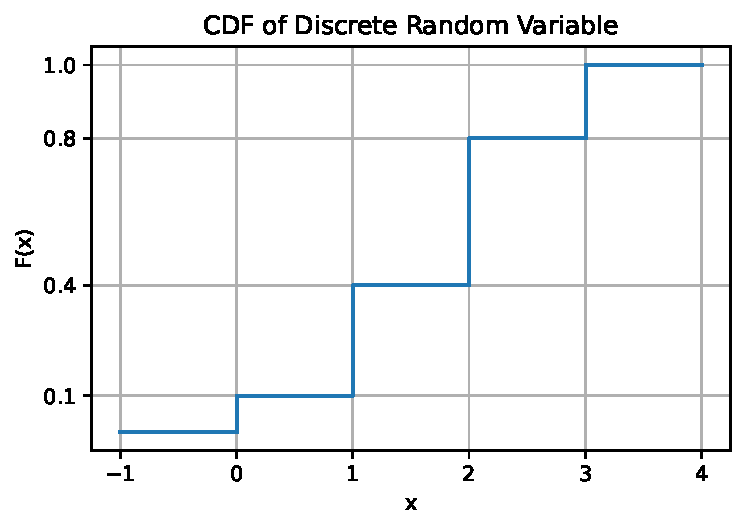
\includegraphics[keepaspectratio]{lec01_files/figure-pdf/cell-2-output-1.pdf}}

Is a step function with jumps at the points where the random variable
takes values.

\begin{tcolorbox}[enhanced jigsaw, opacitybacktitle=0.6, bottomtitle=1mm, opacityback=0, toprule=.15mm, colbacktitle=quarto-callout-note-color!10!white, colback=white, left=2mm, title={Properties of Cumulative Distribution Functions}, breakable, rightrule=.15mm, leftrule=.75mm, titlerule=0mm, colframe=quarto-callout-note-color-frame, arc=.35mm, coltitle=black, toptitle=1mm, bottomrule=.15mm]

\phantomsection\label{properties-cdf}
For any random variable \(X\), its CDF \(F_X(x)\) has the following
properties:

\begin{enumerate}
\def\labelenumi{\arabic{enumi}.}
\tightlist
\item
  \textbf{Monotonicity}: \(F_X(x)\) is non-decreasing. For any
  \(x_1 < x_2\), \(F_X(x_1) \le F_X(x_2)\).
\item
  \textbf{Limits}: \(\lim_{x \to -\infty} F_X(x) = 0\) and
  \(\lim_{x \to \infty} F_X(x) = 1\).
\item
  \textbf{Right-continuity}: \(F_X(x)\) is right-continuous, meaning
  \(\lim_{h \to 0^+} F_X(x+h) = F_X(x)\) for all \(x\).
\end{enumerate}

\end{tcolorbox}

The properties above hold for both discrete and continuous random
variables. For discrete random variables, the CDF is a step function
(continuous from the right), while for continuous random variables, the
CDF is a continuous function.

\begin{tcolorbox}[enhanced jigsaw, opacitybacktitle=0.6, bottomtitle=1mm, opacityback=0, toprule=.15mm, colbacktitle=quarto-callout-note-color!10!white, colback=white, left=2mm, title={CDF of a continuous random variable}, breakable, rightrule=.15mm, leftrule=.75mm, titlerule=0mm, colframe=quarto-callout-note-color-frame, arc=.35mm, coltitle=black, toptitle=1mm, bottomrule=.15mm]

\begin{example}[]\protect\hypertarget{exm-cdf-continuous}{}\label{exm-cdf-continuous}

Consider a random variable \(X\) representing the time (in hours) a
server remains operational before crashing. \(X\) can take any
non-negative real value. Assume the probability density function (pdf)
is given by: \[
f_X(x)=
\begin{cases}
\frac{1}{100} e^{-x/100} & \text{if } x \ge 0 \\
\rule{0in}{3ex}0 & \text{if } x < 0
\end{cases}
\]

This probability distribution is called an \textbf{exponential
distribution with a mean of 100 hours}. We will define and talk about
mean later. The CDF is computed as follows:

\[
F_X(x) = P(X \le x) = \int_{-\infty}^x f_X(t) dt =
\begin{cases}
0 & \text{if } x < 0 \\
1 - e^{-x/100} & \text{if } x \ge 0
\end{cases}
\]

The CDF \(F_Y(y) = P(Y \le y)\) would give the probability that the
server operates for at most \(y\) hours. For instance, \(F_Y(10)\) would
be the probability the server fails within the first 10 hours.

\end{example}

\end{tcolorbox}




\end{document}
